\chapter{PCB
\index{Chapter!PCB}
\index{PCB}
\label{PCB}}
\section{Schematic}
\subsection{ORCad Capture Overview}
ORCad comes with a schematic software called Capture CIS which we used to create our schematics. As a reference to both us and others, this section is
dedicated to providing a small walkthrough to using the software and some nice-to-know features.
\begin{figure}[H]
  \centering
  \scalebox{.3}{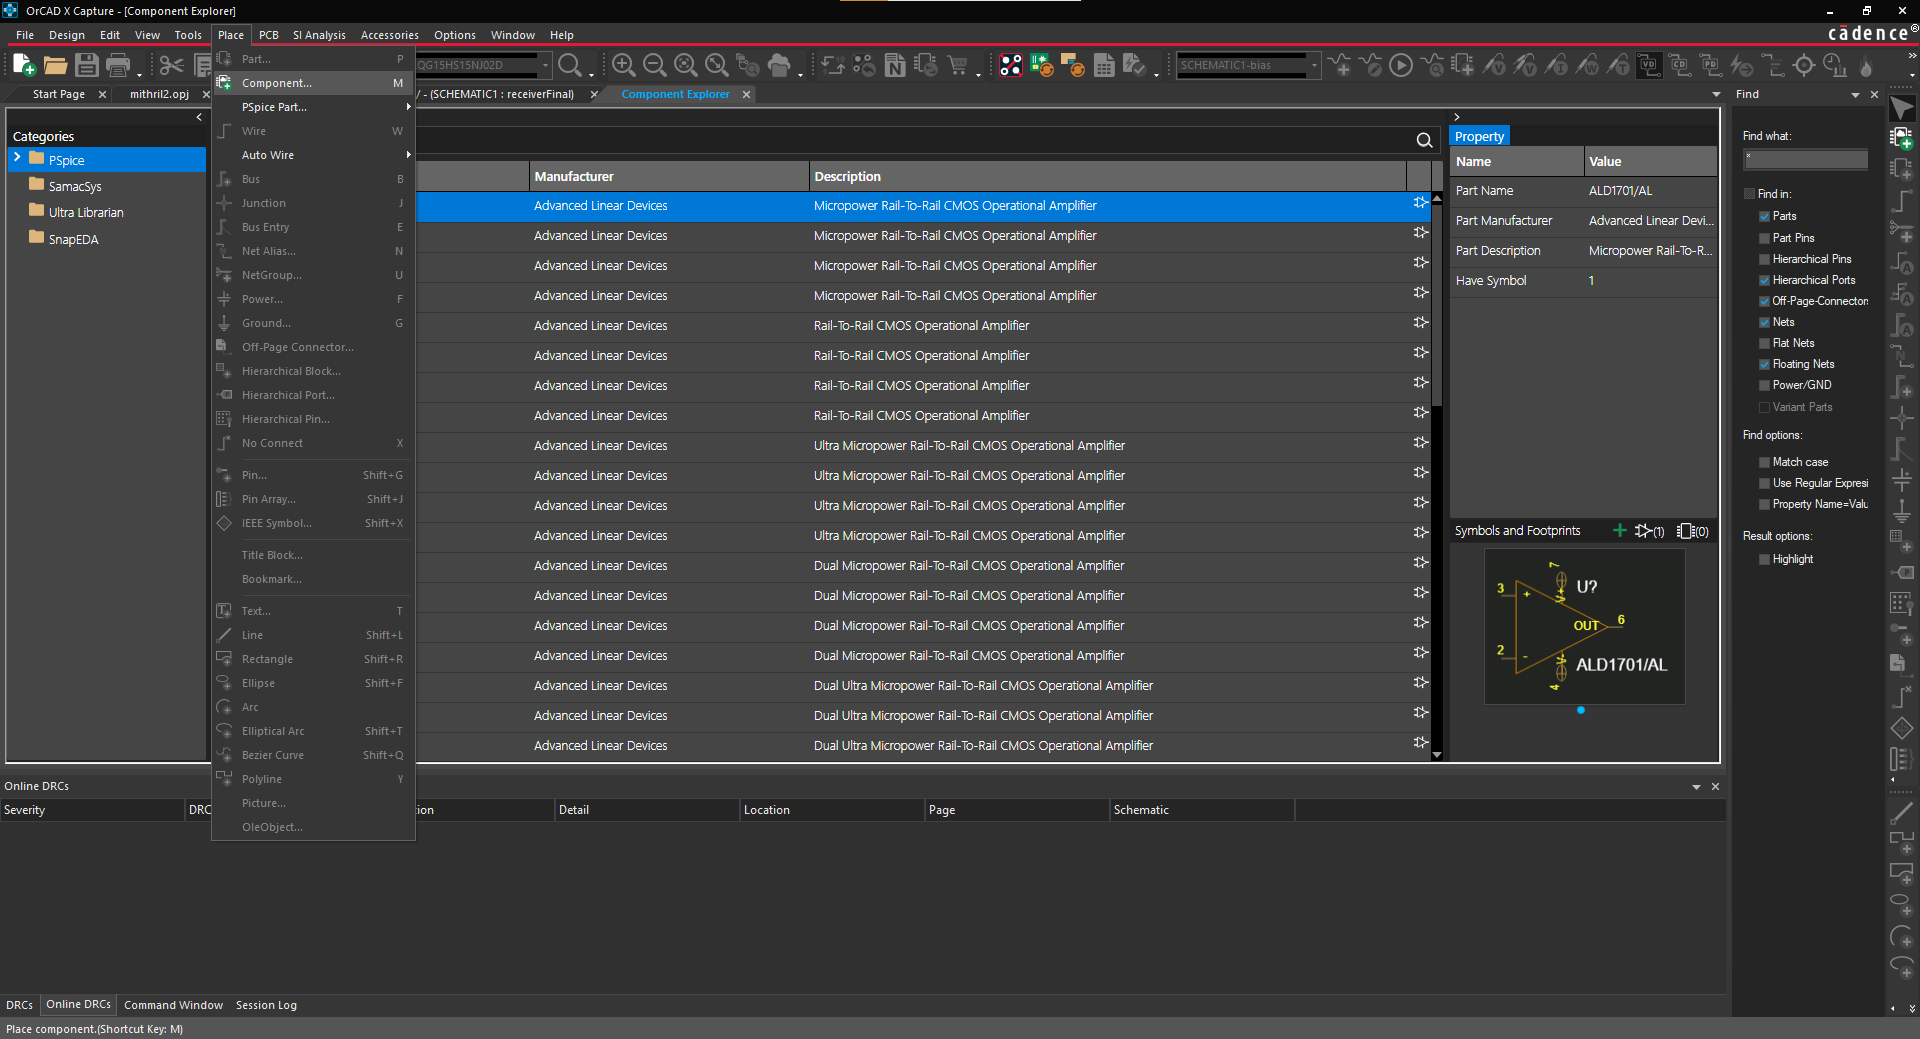
\includegraphics{CaptureImages/ultralib.png}}
\caption{Component Database Search}
\label{img:ultralib}
\end{figure}

The first important feature we found was the component database, which can be seen in Figure \ref{img:ultralib}. By clicking on the icon that has a small chip and cloud will 
take you to this page which contains subdirectories "PSpice" "SamacSys" "UltraLibrarian" and "SnapEDA". PSpice contains parts that
have simulation properties, but we ignored this as we did not know how to use PSpice. The other three are different databases
containing schematic symbols and layout footprints for parts that can be found on major retailers like DigiKey, Mouser, and Arrow.

\begin{figure}[H]
  \centering
  \scalebox{.5}{
\includegraphics{CaptureImages/ultralibexample.png}}
\caption{Schematic/Footprint Examples}
\label{img:ultralibexample}
\end{figure}

You can search for parts in the search fields for the different databases to try to find a part that has a schematic symbol
and footprint available. You can see in Figure \ref{img:ultralibexample} that parts with the symbol and footprint available will
have an amp and chip symbol next to them. The box means there is a 3D CAD model associated with them too. If you cannot find
the symbol and footprint for a part, we recommend going on Mouser and finding the part, then requesting the symbol and footprint.
Usually, the schematic and footprint will be added to SamacSys after a couple of days.

\begin{figure}[H]
  \centering
  \scalebox{.3}{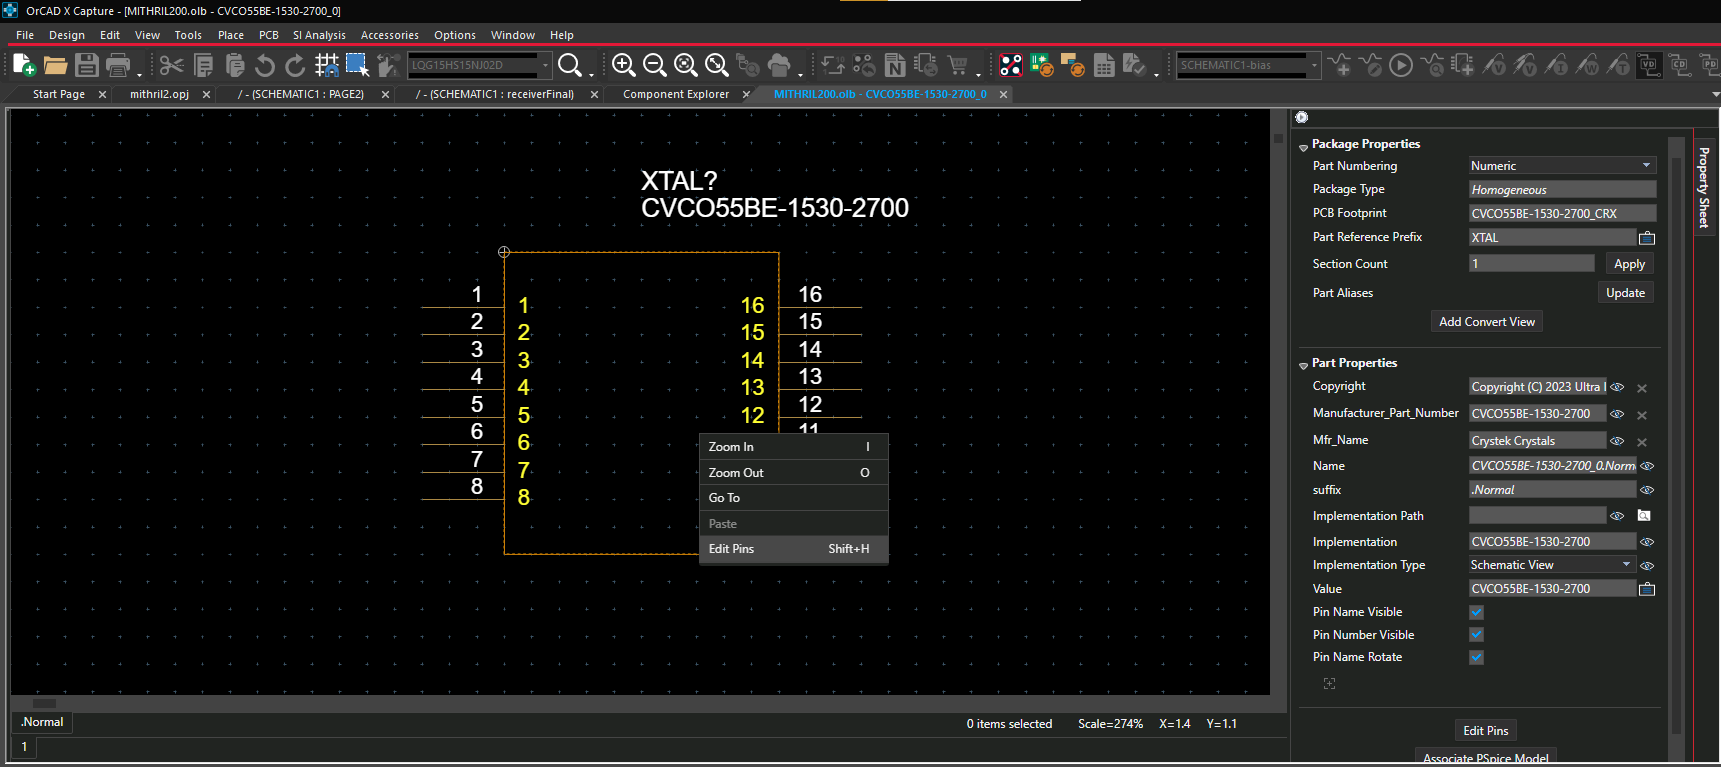
\includegraphics{CaptureImages/editpin.png}}
\caption{Editing Schematic Parts}
\label{img:editpart}
\end{figure}

Sometimes, these symbols and footprints are not correct. If the schematic symbol is incorrectly labeled, you can edit the part,
then click edit pins to make sure all the pins are correctly labeled and numbered as can be seen in Figure \ref{img:editpart}.

\begin{figure}[H]
  \centering
  \scalebox{.3}{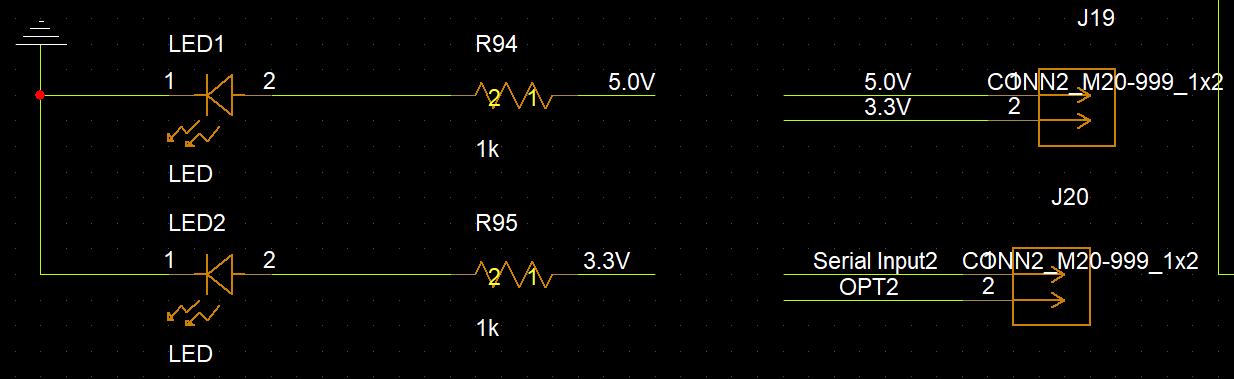
\includegraphics{CaptureImages/wirealias.png}}
\caption{Wires and Net Alias}
\label{img:wirealias}
\end{figure}

Once you've placed your parts down in the schematic, now comes time to connect everything together. To navigate through the
schematic interface, you can use CTRL+Scroll Wheel to zoom in and out, and middle mouse button to scroll left to right.

You can use "w" to enter wiring mode, which lets you place down wires according to your grid size. After wiring, be sure to use
"n" to enter net alias mode and assign aliases to your wires. As can be seen in Figure \ref{img:wirealias}, there are two
non-connected wires both with the alias "5.0V". This effectively connects them since they are under the same alias and will also
label them in the layout when routing. Using the net alias helps with things like power where connecting everything that needs
power with a wire to your power source would make the schematic a mess. In short, all wires with the same net alias are considered
connected.

\begin{figure}[H]
  \centering
  \scalebox{.3}{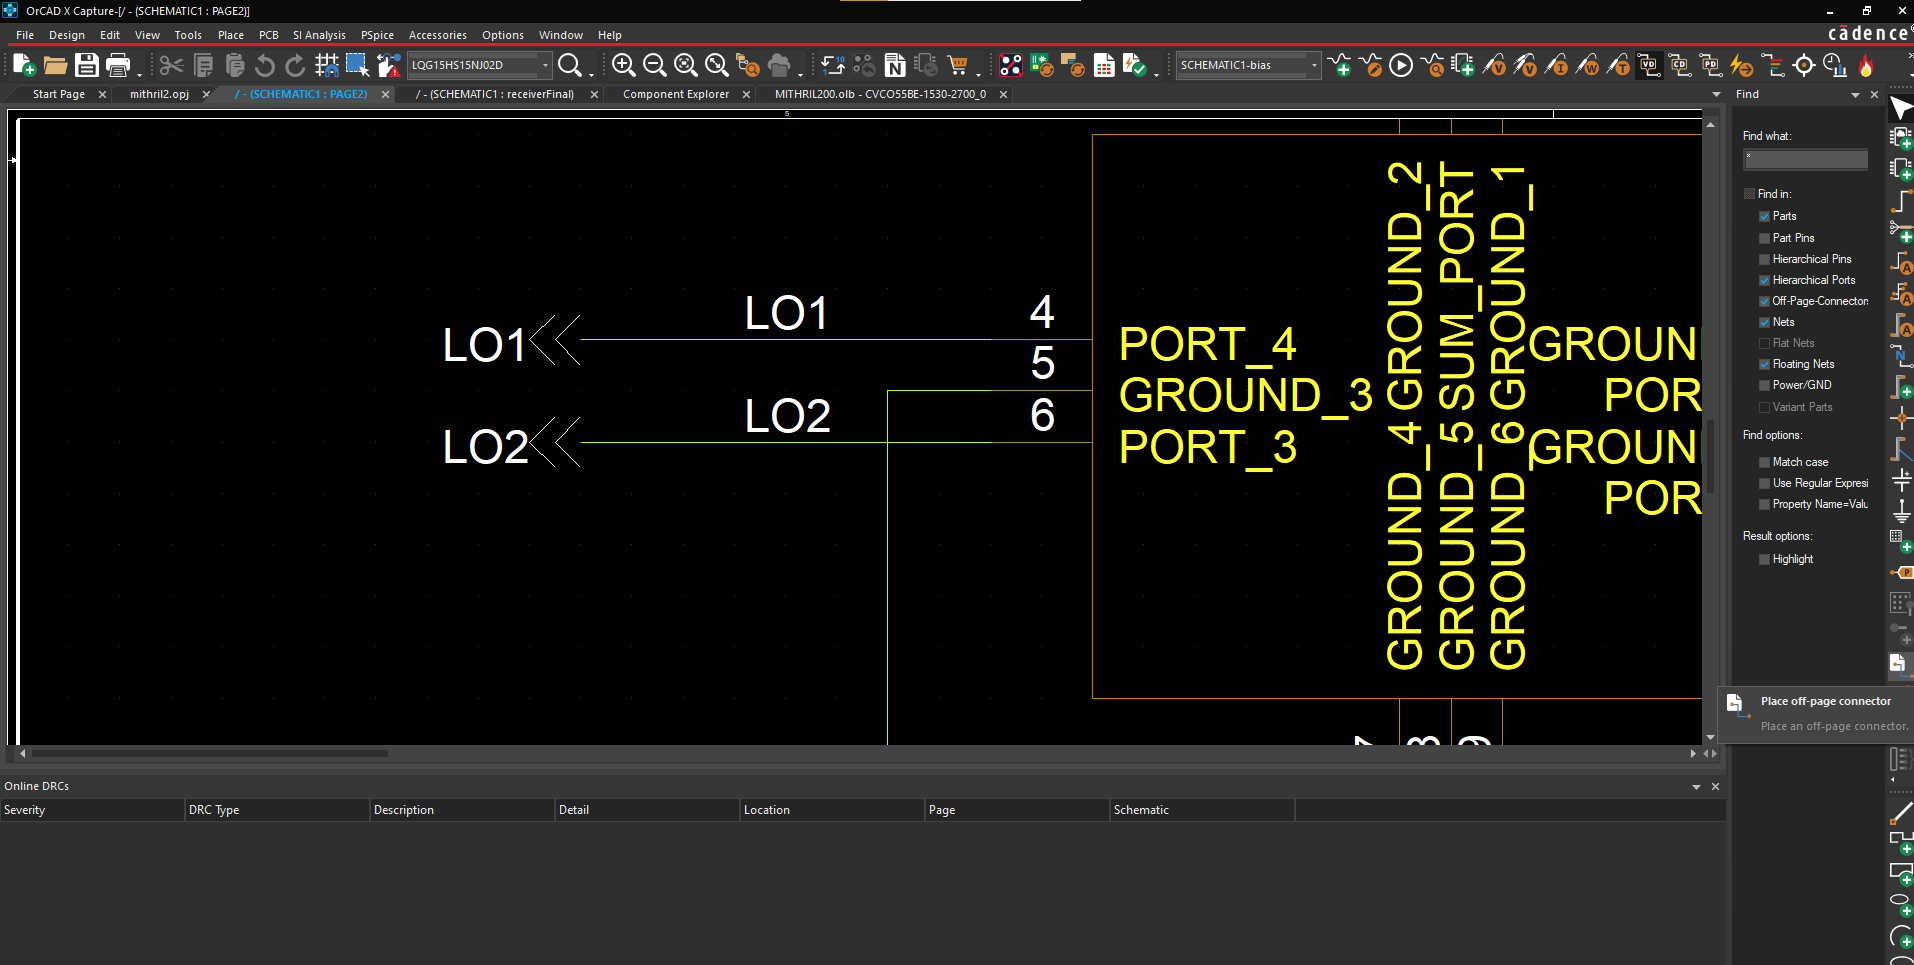
\includegraphics{CaptureImages/offpageconn.png}}
\caption{Off Page Connectors}
\label{img:offpageconn}
\end{figure}

If you run out of room or want to separate your schematics into different pages, you can connect wires from different schematic
pages using off-page connectors as shown in Figure \ref{img:offpageconn}. Connect the off-page connector to a wire and name it
the same on both schematic pages to have the wires connect.

\subsection{Circuitry Good Practices}
\subsubsection{DC Blocking and Coupling Caps}
\begin{figure}[H]
  \begin{minipage}{0.5\textwidth}
    \centering
    \scalebox{.3}{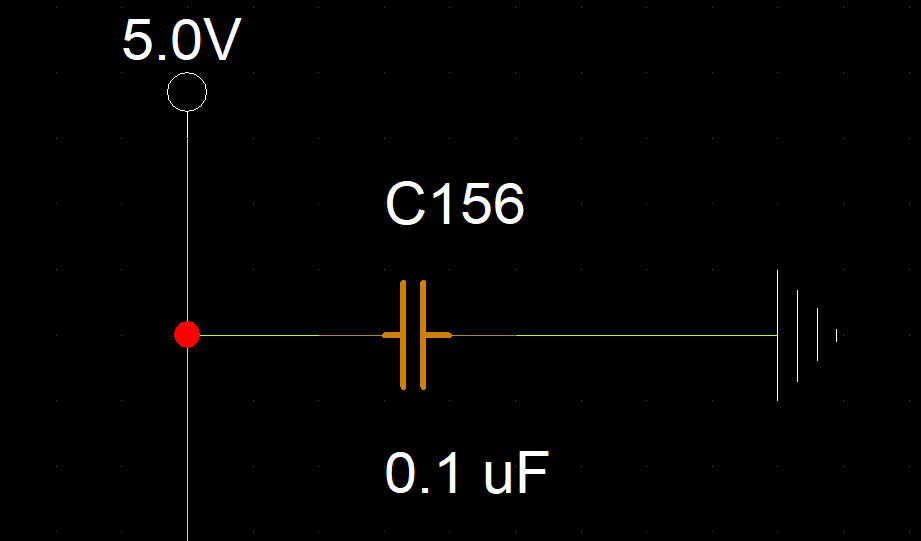
\includegraphics{CaptureImages/coupling.png}}
    \caption{Coupling Capacitor}
    \label{img:couplingcap}
  \end{minipage}
  \begin{minipage}{0.5\textwidth}
    \centering
    \scalebox{.3}{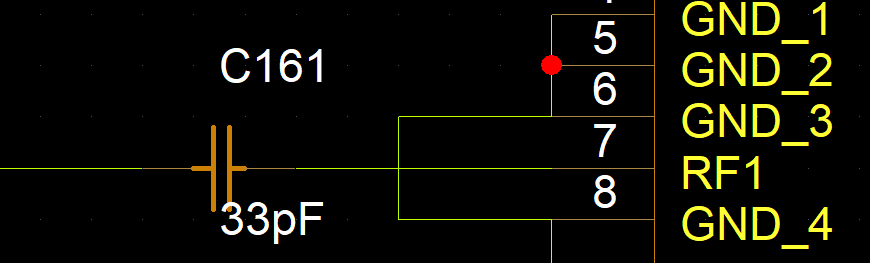
\includegraphics{CaptureImages/dcblocking.png}}
    \caption{DC Blocking Capacitor}
    \label{img:dcblockingcap}
  \end{minipage}
\end{figure}

Two good practices to include in your schematics are coupling and DC blocking capacitors. 

Coupling capacitors are usually used when giving power to some component or chip as can be seen in Figure \ref{img:couplingcap}. It 
can be thought of as a mini low-pass filter, where the capacitance of your coupling capacitor will affect the 
cutoff frequency of the filter. These coupling capacitors should be placed in parallel with the power wire that goes into the chip.

DC Blocking capacitors do the exact opposite, and are usually used when passing a signal from one component to another as can be 
seen in Figure \ref{img:dcblockingcap}. They can be thought of as mini high-pass filters, where the capacitance of the DC Blocking
capacitor affects the cutoff frequency. These are placed in series with the signal wire.
\begin{figure}[H]
\begin{equation}
  C = \frac{1}{2\pi Xf}
  \end{equation}
  \caption{Capacitance of a Coupling or DC Blocking Capacitor}
  \label{eq:capacitance}
\end{figure}
The equation for finding the capacitance of either the coupling or DC blocking capacitor can be seen in Equation \ref{eq:capacitance} 
where C is the capacitance, X is the impedance, and f is the cutoff frequency.
Essentially, a higher cutoff frequency corresponds to a lower capacitance value, and the only difference between the coupling and
DC blocking capacitor is the coupling capacitor passes everything below that cutoff frequency, and the DC blocking capacitor passes
everything above that cutoff frequency.
\subsubsection{Test Pins and Grounds}
\begin{figure}[H]
  \centering
  \scalebox{.3}{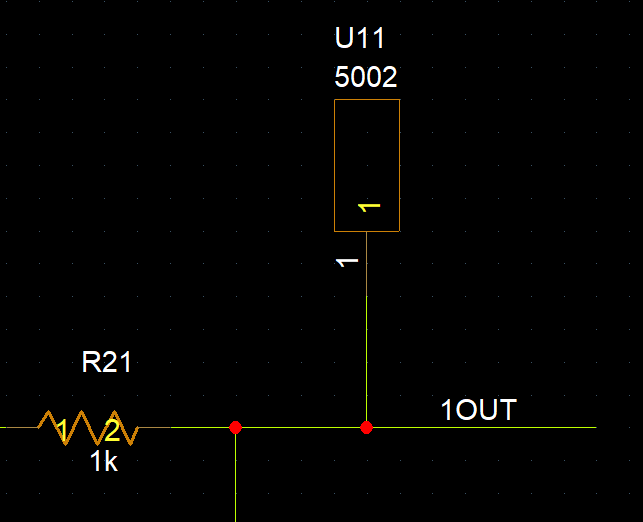
\includegraphics{CaptureImages/testpin.png}}
\caption{Test Pin}
\label{img:testpin}
\end{figure}

Other extremely important things to add are test pins as seen in Figure \ref{img:testpin} and exposures to ground. Credit to
Professor Muresan for telling us to add both of these as they were vital to testing and the operation of the board.

Test pins should be placed in parallel with signal wires so that you can hook in with an oscilloscope and examine what is happening.
Really, after every stage in a signal chain it would be good practice to expose the signal via a test pin or if it is RF with an
SMA connector. This allows you to debug analog things and find out how each stage is affecting your signal. We only added it
in one place and after the fact wished we had placed more test pins so we could see what was happening from component to component.

Ground pins and pads are also really important. We overlooked adding a ground pin which was extremely inconvenient for us, and wished we
had put ample ground pins and pads everywhere on the board. These are necessary if using external components with the board, since
they should have a common ground.

\subsubsection{Power LEDs}
\begin{figure}[H]
  \centering
  \scalebox{.3}{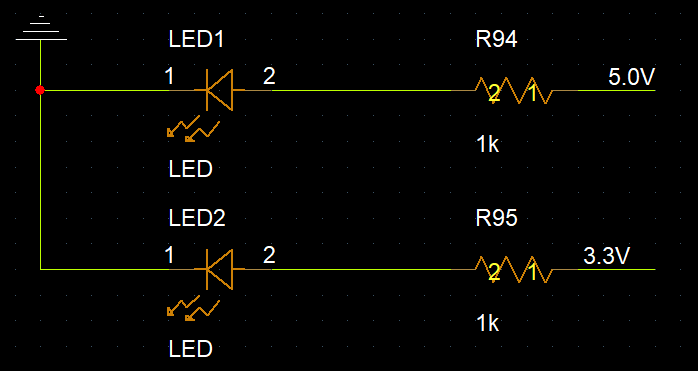
\includegraphics{CaptureImages/leds.png}}
\caption{Power LEDs}
\label{img:led}
\end{figure}

Another nice thing to have are some LEDs connected to power, just so you know at the very least your board is turned on and everything
is receiving power. Having a switch of some sort to block power is also something nice to have which we did not add.

\subsubsection{Potentiometers}
\begin{figure}[H]
  \centering
  \scalebox{.3}{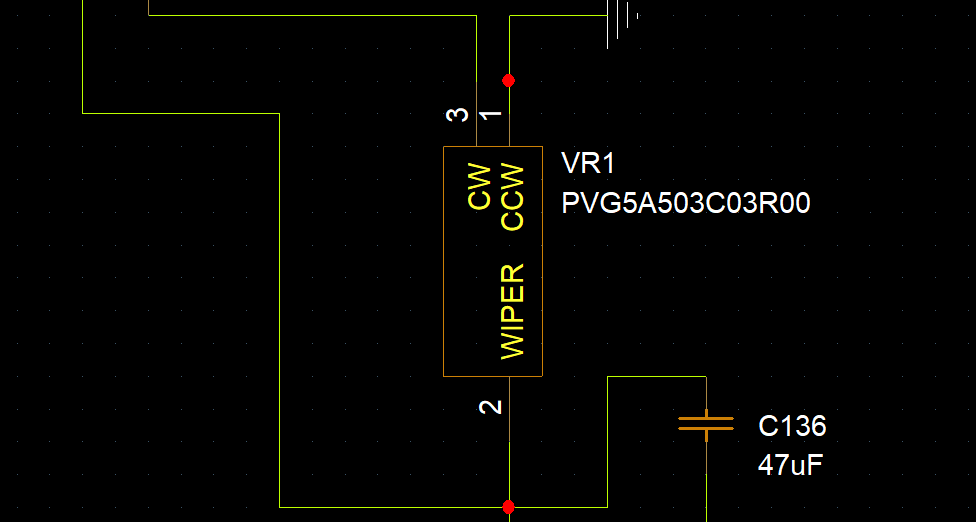
\includegraphics{CaptureImages/pot.png}}
\caption{Potentiometers}
\label{img:pot}
\end{figure}

Another extremely useful thing to add is potentiometers, as can be seen in Figure \ref{img:pot}. In things like amplifying or
filtering stages where resistors can change the cutoff frequency or gain of your circuit, potentiometers are very useful. From
Figure \ref{img:pot}, we can see that potentiometers have three ports: CCW, CW, and Wiper. How potentiometers work is that the
wiper controls the resistance of the potentiometer, and turning it CW will make more signal go in that port, and turning it CCW will
make more signal go into that port (oversimplified explanation). Therefore, it can be set up by just feeding the input to the wiper,
the output to CCW, and CW to ground. This can help with changing gains and cutoff frequencies even after the board is printed and
assembled.

\subsection{Transmitter}
\begin{figure}[H]
  \centering
  \scalebox{.5}{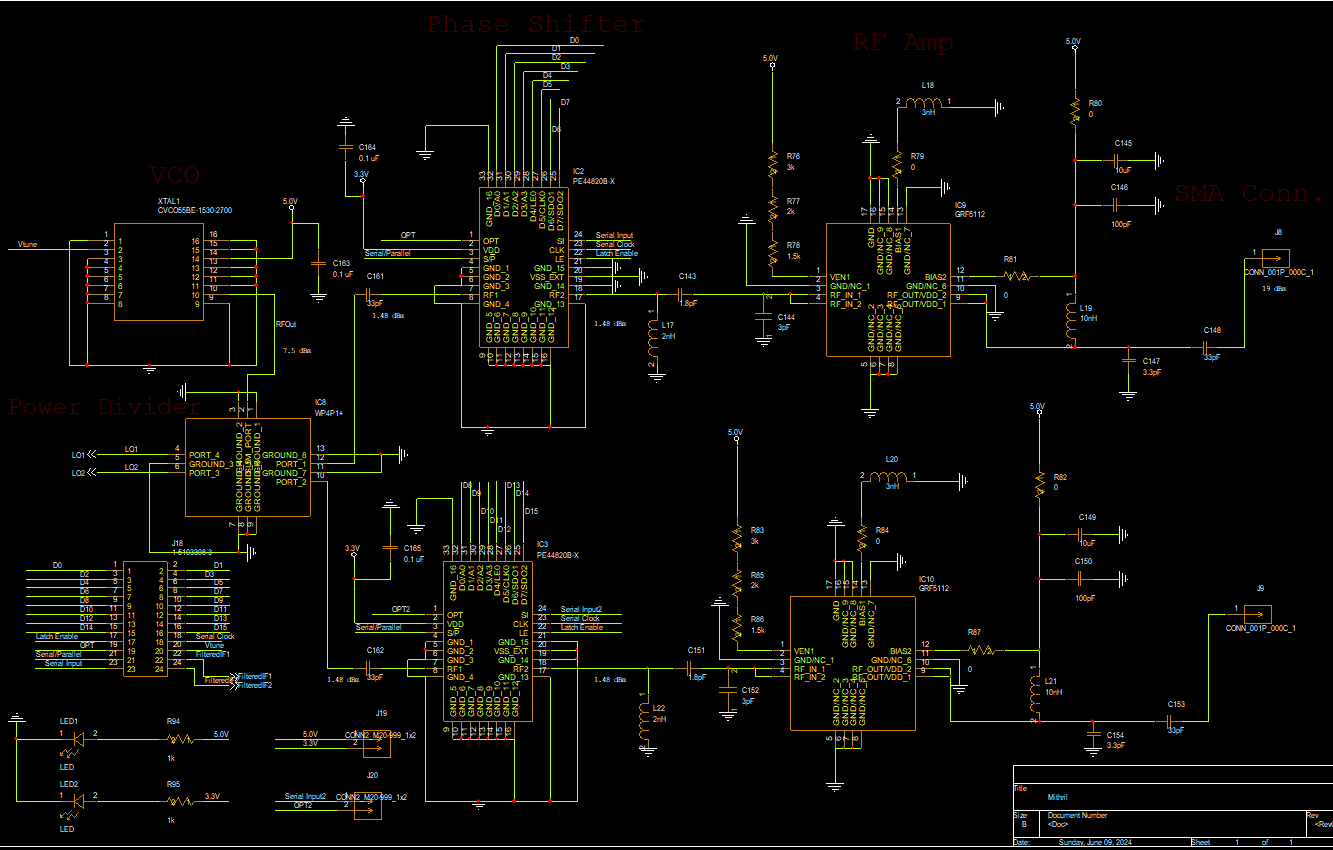
\includegraphics{CaptureImages/transmitterfull.png}}
\caption{Transmitter Schematic}
\label{img:transmitterfull}
\end{figure}
The first step in creating a PCB is fleshing out the schematic. We already decided on what parts to use in Chapter \ref{Part Selection},
and now was the time to create a circuit which interfaces the parts together to make a fully functioning system.
As can be seen in Figure \ref{img:transmitterfull}, the stages of the RF chain are labeled reflecting what was discussed in the
Part Selection chapter. Essentially all of the parts shown here are connected to resistors, capacitors, and inductors according
to the example schematics in their respective datasheets. In the bottom left of the schematic we can see some LEDs
that are connected to power just to make sure the board is being powered and our GPIO connector which will be used to control our
parts. 

The signal path starts with synthesis at the VCO. The VCO connects to 5 volts and is controlled by a tuning voltage will
determine the frequency at the output port of the VCO. This Vtune wire is connected to the GPIO header.

This output signal is then connected to a power divider which splits it four ways. Two of the split signals will
go to the next stage in the RF chain, and the other two are used as local oscillators in the receiver chain. 
This can be seen by two ports of the power divider being connected to off page connectors which can be accessed by the
receiver in another schematic page.

The next stage of the RF chain in the transmitter portion are the phase shifters. The phase shifters will change the phase
of the two identical signals which essentially means a time delay. This causes construction and destruction when the
two signals propogate through the air, and allows for concentrated energy in one direction. We chose 8 bit digital 
phase shifters that have both a serial and parallel interface. The part is connected to 3.3 volts, and has a lot of control and
data pins that we connected to our GPIO header to allow for control by our microcontroller. The phase shifter and its
operation will be discussed more in Chapter \ref{Digital Processing}. 

Finally, the signal passes through our power amplifier with a small signal gain of 17.1 dBm which should help it propogate
through the air for a longer period of time without dissipating. The amplified signal will then propogate through two transmitting
antennas (our small phased array of antennas) to construct and destruct forming a beam of EMF.

\subsection{Receiver}
\begin{figure}[H]
  \centering
  \scalebox{.5}{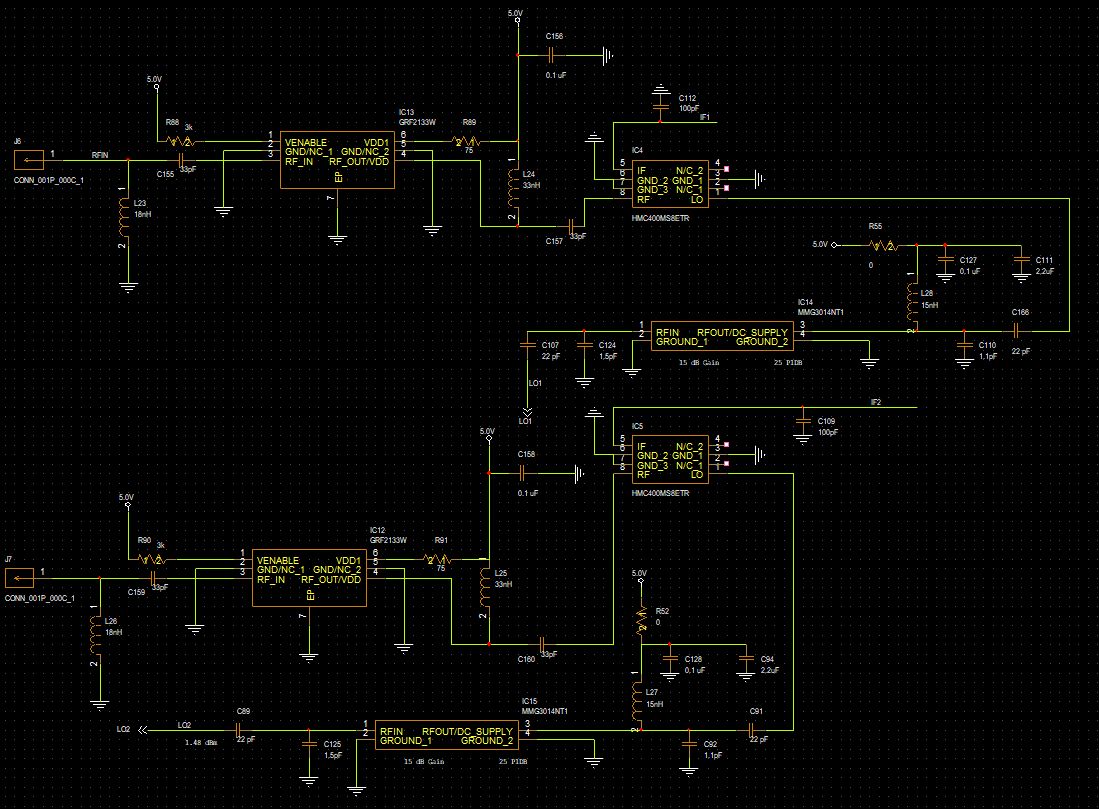
\includegraphics{CaptureImages/receiverfull.png}}
\caption{RF Portion of Receiver Schematic}
\label{img:receiverschem}
\end{figure}
After our signal propogates through the air, it should hit some objects and reflect back to the physical system, and the
goal is to capture this signal and make it digestible to analyze. The first step is capturing the signal, which is accomplished
through the RF portion of the receiving schematic shown in Figure \ref{img:receiverschem}.

First, we have two receiving antennas where the reflected signal should induce a signal in the antennas. We have two
receiving antennas to distinguish the angle of arrival as discussed in \ref{Radar Theory}.

The very small signal induced in the antennas will then pass through a low-noise amplifier which is supposed to amplify our small
signal to be used in the later stages of the chain. The reason a low-noise amplifier is used in a receiving RF chain is because
the first stage of a receiver is the most impactful on its signal-to-noise ratio, or how strong the signal has to be to be
distinguishable from noise. This is discussed more in depth in Chapter \ref{Radar Theory}. This part is powered by 5 volts, and
also has an enable pin that can set the gain of the LNA and disable it if need be. There is also a pin called "EP" which stands
for exposed pad. it is essentially a big ground pad that is used as a heat sink, distributing heat to the ground plane.

After being amplified, the signal is fed into a mixer. The mixer is supposed to output the sum and difference of two RF signals.
One of these is our amplified return signal, the other is a copy of out transmitted signal (LO). This transmitted signal comes from
an off-page connector which is connected to the power divider in the transmitter schematic, and is then amplified by a power
amplifier according to the mixer's LO specifications. The reason it is amplified is because the mixer is a passive
component, meaning it does not use an external power source for its functionality.
The mixer feeds these signals into the RF and LO ports respectively, and
outputs the sum and difference of these signals out of the IF or intermediate frequency port.

\begin{figure}[H]
  \centering
  \scalebox{.5}{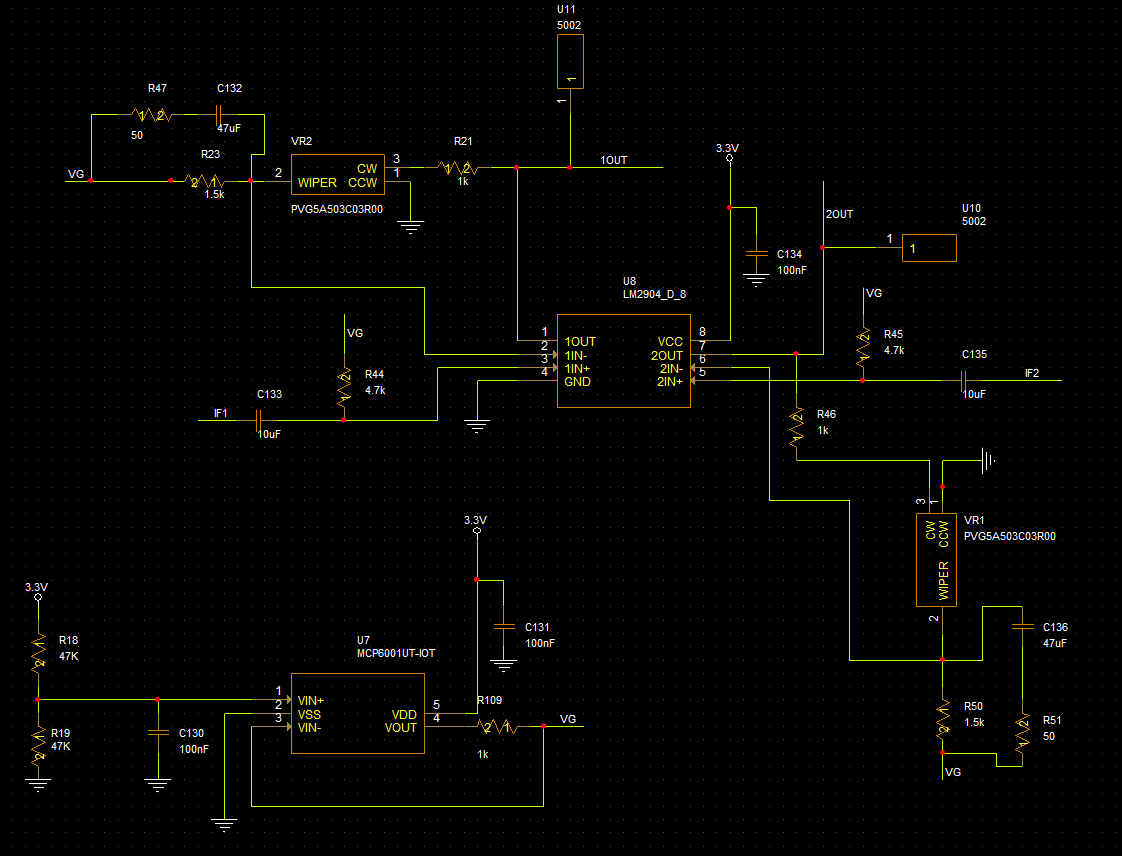
\includegraphics{CaptureImages/basebandamp.png}}
\caption{IF Amplifier Stage}
\label{img:ifamplifier}
\end{figure}

After the sum and difference of our VCO copy (Local Oscillator) and return signal
are outputted from the mixer, we need to do some post-processing to make sense of it.
The first stage of the intermediate frequency processing is in our case
amplification (which turned out to be a bad idea as can be seen in Chapter \ref{Issues}).
As mentioned in \ref{Part Selection}, our mixers output has a reference of 0v or ground.
This means that it contains positive and negative voltage as part of its signal. However,
we decided to use single supply amplifiers. This means its theoretical rails are 0v (ground)
to Vcc (3.3v in this case). Therefore, we need to bias our mixer output around the middle of our rails
to avoid clipping and to take advantage of the full bandwidth of the amp.

The bottom left of Figure \ref{img:ifamplifier} shows our biasing circuit,
which is a simple voltage division using equal resistors and a voltage follower
to keep the voltage steady. This becomes our new "virtual ground", or reference voltage
when dealing with the amplifier. Looking at the dual amp in the center of Figure \ref{img:ifamplifier}, we can see that the mixer output (labeled IF1 and IF2) is
biased with our DC voltage from the biasing circuit, effectively making the new reference 3.3/2 volts. 

\begin{figure}[H]
  \centering
  \scalebox{.5}{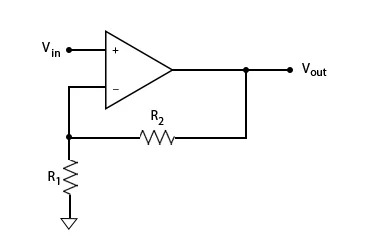
\includegraphics{Diagrams/non-inverting-amp.jpg}}
\caption{Non-Inverting Amplifier Circuit}
\label{img:noninverting}
\end{figure}

The amplifier setup itself was taken from a Finnish engineer named Henrik Forsten whose blog we followed closely and can be found
\href{https://hforsten.com/6-ghz-frequency-modulated-radar.html}{here}. Essentially, it follows a basic non-inverting amplifier
circuit which can be seen in Figure \ref{img:noninverting}. The output of the amplifier feeds to a potentiometer (R2), 
and shares a node with resistance tied to ground (R1) and the negative input of the amplifier. The potentiometer makes this
a variable-gain amplifier, since we can change R2 to different resistance values to fine tune the amplification based on how
small or large the mixer's output is. The ground for the power supply in the amplifier is connected to the power supply, but 
we simply replaced everywhere there would have been ground in the rest of the circuit with our "virtual ground" from the biasing circuit
to make the reference 3.3/2 volts.

\begin{figure}[H]
  \centering
  \scalebox{.5}{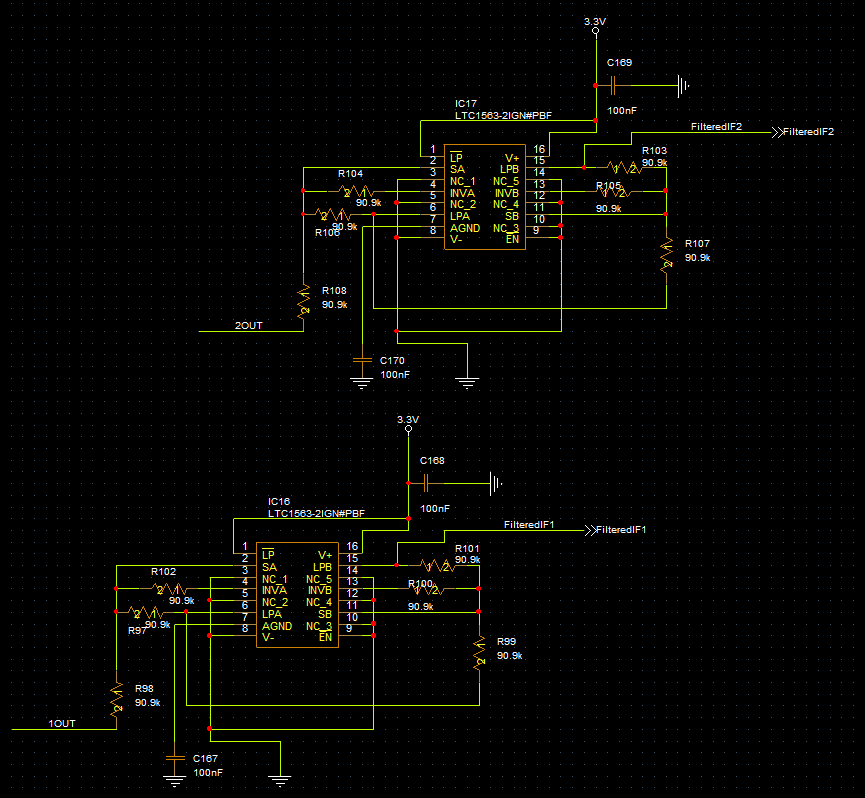
\includegraphics{CaptureImages/filters.png}}
\caption{Low Pass Filters}
\label{img:lpf}
\end{figure}

At this point, our intermediate frequency signal is amplified, but might still have
noise from the antenna or high frequency components from the mixer. In order to remove
these unwanted frequencies from our signal, we want to apply some filtering to only leave
the intermediate frequency of interest. We added fourth-order butterworth LPFs after
the amplifiers to attenuate these other signals. As we can see in \ref{img:lpf}, the 
chip takes multiple resistance values that determine its cutoff frequency.

\begin{figure}[H]
  \begin{equation}
    R = 10k \left(\frac{256kHz}{f_C}\right); \quad f_C = \text{Cutoff Frequency}
    \end{equation}
    \caption{Cutoff Frequency Equation for LPF}
    \label{eq:LPF}
  \end{figure}

The resistances can be determined by Equation \ref{eq:LPF}, and in our case
we used 90.9k resistors to achieve a cutoff frequency of 28 kHz. This filtered
signal then goes to a GPIO pin which will be sampled by a microcontroller.

\section{Layout}
\